\documentclass[a4paper,12pt]{jarticle}

% レイアウト
%---------------------------------------------
\setlength{\hoffset}{0cm}
\setlength{\oddsidemargin}{-3mm}
\setlength{\evensidemargin}{-3cm}
\setlength{\marginparsep}{0cm}
\setlength{\marginparwidth}{0cm}
\setlength{\textheight}{24.7cm}
\setlength{\textwidth}{17cm}
\setlength{\topmargin}{-45pt}
%---------------------------------------------
\renewcommand{\baselinestretch}{1.2}
\renewcommand{\floatpagefraction}{1}
\renewcommand{\topfraction}{1}
\renewcommand{\bottomfraction}{1}
\renewcommand{\textfraction}{0}
\renewcommand\thefootnote{\arabic{footnote})}
%---------------------------------------------
% パッケージ
%---------------------------------------------
\usepackage[dvipdfmx]{graphicx}
\usepackage{amsmath,amssymb,epsfig}
\usepackage{eucal}
\usepackage{bm}
\usepackage{ascmac}
\usepackage{pifont}
\usepackage{multirow}
\usepackage{enumerate}
\usepackage{cases}
\usepackage{type1cm}
\usepackage{cancel}
\usepackage{url}
\usepackage{cite}
%\usepackage{color}
\usepackage[dvipdfmx]{color}
\usepackage{caption}
\usepackage[caption=false]{subfig}
\captionsetup[figure]{labelsep=space}
\usepackage{verbatim}
%\usepackage{listings,jlisting}
%---------------------------------------------
% 擬似コード作成用
%---------------------------------------------
\usepackage[ruled,vlined]{algorithm2e}
\usepackage{setspace}
\input{../sty/jdummy.def}
%---------------------------------------------
% カウンタの設定
%---------------------------------------------
\setcounter{section}{0}
\setcounter{subsection}{0}
\setcounter{subsubsection}{0}
\setcounter{equation}{0}
%---------------------------------------------
% キャプションの図をFigに変更
%---------------------------------------------
\renewcommand{\figurename}{Fig.}
\renewcommand{\tablename}{Tab.}
%---------------------------------------------
% 式番号を式(章番号.番号)に
%---------------------------------------------
\makeatletter
\renewcommand{\theequation}{\arabic{section}.\arabic{equation}}
% \renewcommand{\theequation}{\arabic{equation}}
\@addtoreset{equation}{section}
\makeatother
%---------------------------------------------
% 表紙
\title{\vspace{5mm}\\
\Large{車両制御特論\\レポート1\\}
% {\large No title}
}
\author{\vspace{80mm}\\
九州工業大学\ \hspace{0mm} 工学府\\
機械知能工学専攻\ \hspace{0mm} 知能制御工学コース\\
\\
所属:\ 西田研究室\\
学籍番号:\ 17344219\\
提出者氏名:\ 二宮 \hspace{0mm} 悠二\\\vspace{5mm}\\}
\date{平成29年\ 7月\ 12日}
%---------------------------------------------
% ドキュメントの開始
\begin{document}
%---------------------------------------------
% 表紙
\titlepage
\maketitle
\thispagestyle{empty}
\newpage
%---------------------------------------------
% 目次
\thispagestyle{empty}
\tableofcontents
\newpage
%---------------------------------------------
% 課題内容
%---------------------------------------------
\section{課題内容}
%---------------------------------------------
本課題では,次のシステムの応答を解析する.
MATLAB/Simulink にてシミュレーションを行い,解析的に求めた解との比較を行う.
%---------------------------------------------
\begin{equation}
 \dot{x}(t) = -4 x(t) + 8 u_2(t), ~~ x(0) = -5, ~~ u_2(t) = 2 + {\rm cos} ~ t
\label{1}
\end{equation}
%---------------------------------------------
\section{解析的解の導出}
%---------------------------------------------
1節に示したシステムの解析解を導出する.式(\ref{1})の両辺を$ {\cal L}[x(t)] = X(s) $としてラプラス変換すると,
%---------------------------------------------
\begin{equation}
 sX(s) - x(0) = -4X(s) + \frac{16}{s} + \frac{8s}{s^2+1} 
\end{equation}
%---------------------------------------------
となる.さらにこの式を$ X(s) $について解くと次のようになる.
%---------------------------------------------
\begin{eqnarray}
 (s + 4)X(s) & = & -5 + \frac{16}{s} +\frac{8s}{s^2+1} \nonumber\\
        X(s) & = & - \frac{5}{s+4} + \dfrac{16}{s} \cdot \dfrac{1}{s+4} + \dfrac{8}{s+4} \cdot \dfrac{s}{s^2+1} 
\end{eqnarray}
%---------------------------------------------
この式の両辺を逆ラプラス変換すると
%---------------------------------------------
\begin{eqnarray}
 x(t) & = & -5e^{-4t} + \int_0^t {16e^{-4(t-\tau)}} d\tau + \int_0^t {8e^{-4(t-\tau)} {\rm cos} ~ t ~} d\tau 
\end{eqnarray}
%---------------------------------------------
となり,これを解くことで解析解として次式を得る.
%---------------------------------------------
\begin{eqnarray}
 x(t) & = & - \dfrac{185}{17}e^{-4t} + \dfrac{8}{17}{\rm sin}~t~ + \dfrac{32}{17}{\rm cos}~t~ + 4
\end{eqnarray}
%---------------------------------------------
%---------------------------------------------
\section{MATLAB/Simulink によるシミュレーション}
%---------------------------------------------
\subsection{モデルの作成}
%---------------------------------------------
式(\ref{1})より,本課題にてシミュレーションを行うシステムのモデルを MATLAB/Simulink にて{\bf Fig.}{\ref{model}}のように設計した.また,解析解と Simulink による応答のグラフを描画するためのプログラムを「plot.m」に示す.
%---------------------------------------------
\begin{figure}[tb]
 \begin{center}
  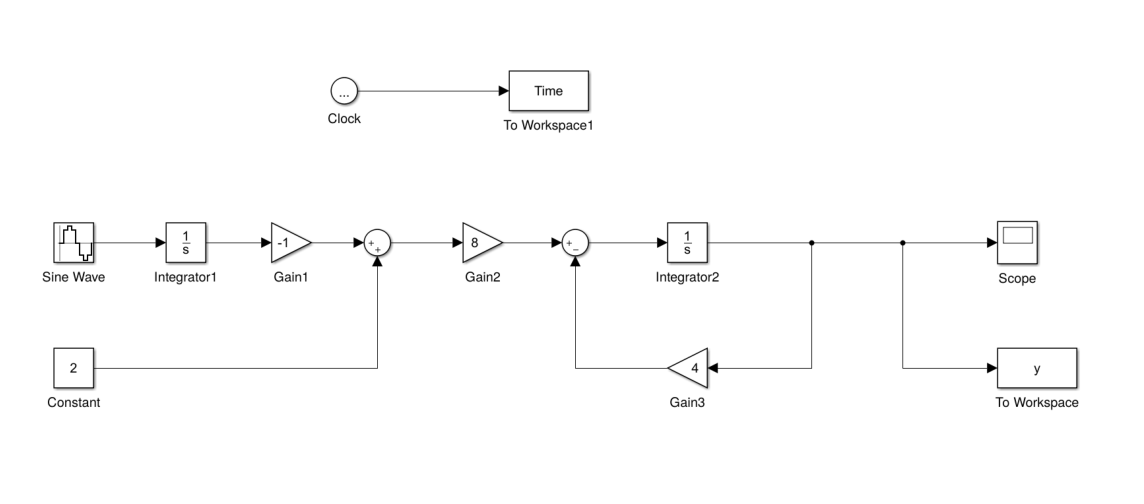
\includegraphics[scale=0.9]{../figure/eps/model2.eps}
  \caption{設計したSimulinkモデル}
  \label{model}
 \end{center}
\end{figure}
%---------------------------------------------
%---------------------------------------------
 %\lstinputlisting{dataplots.m}
% \begin{lstlisting}[caption=作成したMATLABのプログラム]
%   \lstinputlisting{dataplots.m}
% \end{lstlisting}
%---------------------------------------------
\begin{itembox}[l]{plot.m}
 {\scriptsize
 \verbatiminput{dataplots.m}
}
\end{itembox}
%---------------------------------------------
%---------------------------------------------

% \begin{breakbox}
%     \underline{\small M ファイル ``\,{\tt design{\tt \_}k.m}\,'' (コントローラのゲイン $\mbox{\boldmath $K$}$ の算出)}
%     %{\footnotesize \verbatimlisting{dataplot.m}}
% \end{breakbox}
%
%---------------------------------------------
\subsection{シミュレーション結果}
%---------------------------------------------
作成したモデルによる応答および解析解のグラフを出力し,それらを比較したものを{\bf Fig.}\ref{Mat_sim}に示す.
サンプリング周期$ T $は$ T = 0.01 $とした.
%---------------------------------------------
%---------------------------------------------
\begin{figure}[tb]
 \centering
 \subfloat[解析解をプロットしたグラフ]{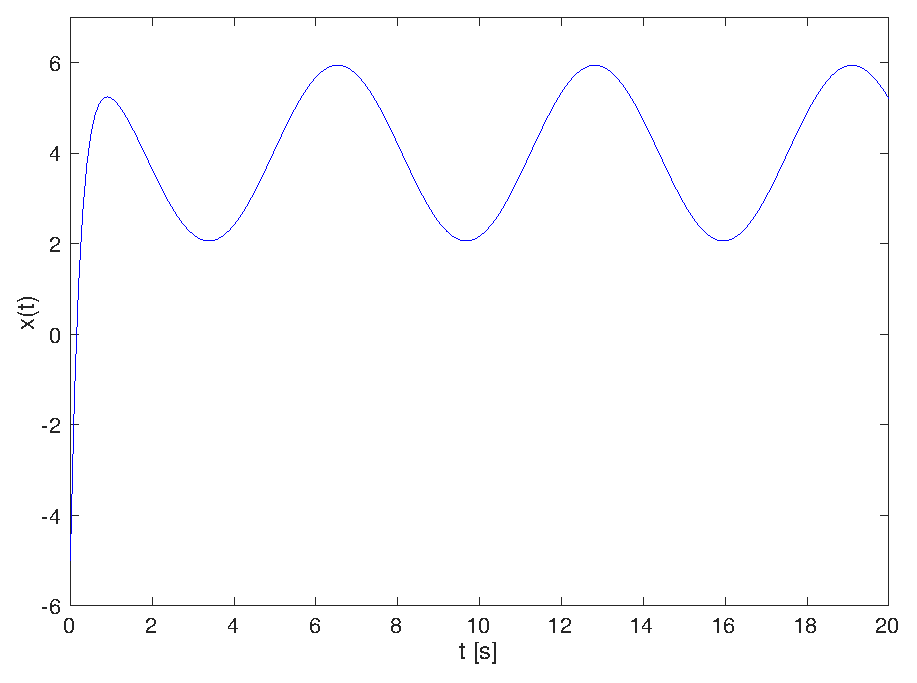
\includegraphics[scale=0.53]{../figure/eps/cali_202.eps}}
 \hspace{1.0cm}
 \subfloat[Simulinkでのシミュレーション結果]{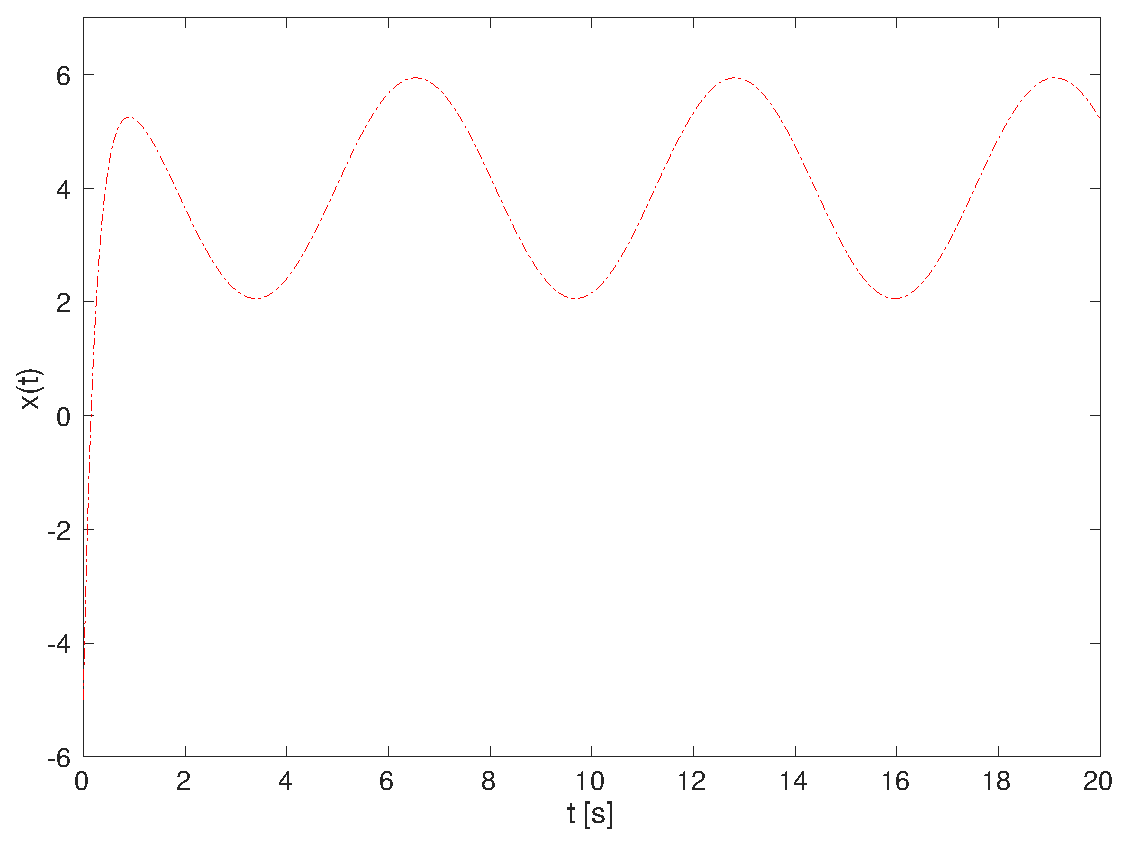
\includegraphics[scale=0.42]{../figure/eps/sim2.eps}}
\\
 \vspace{0.5cm}
 \subfloat[解析解およびシミュレーション結果の比較]{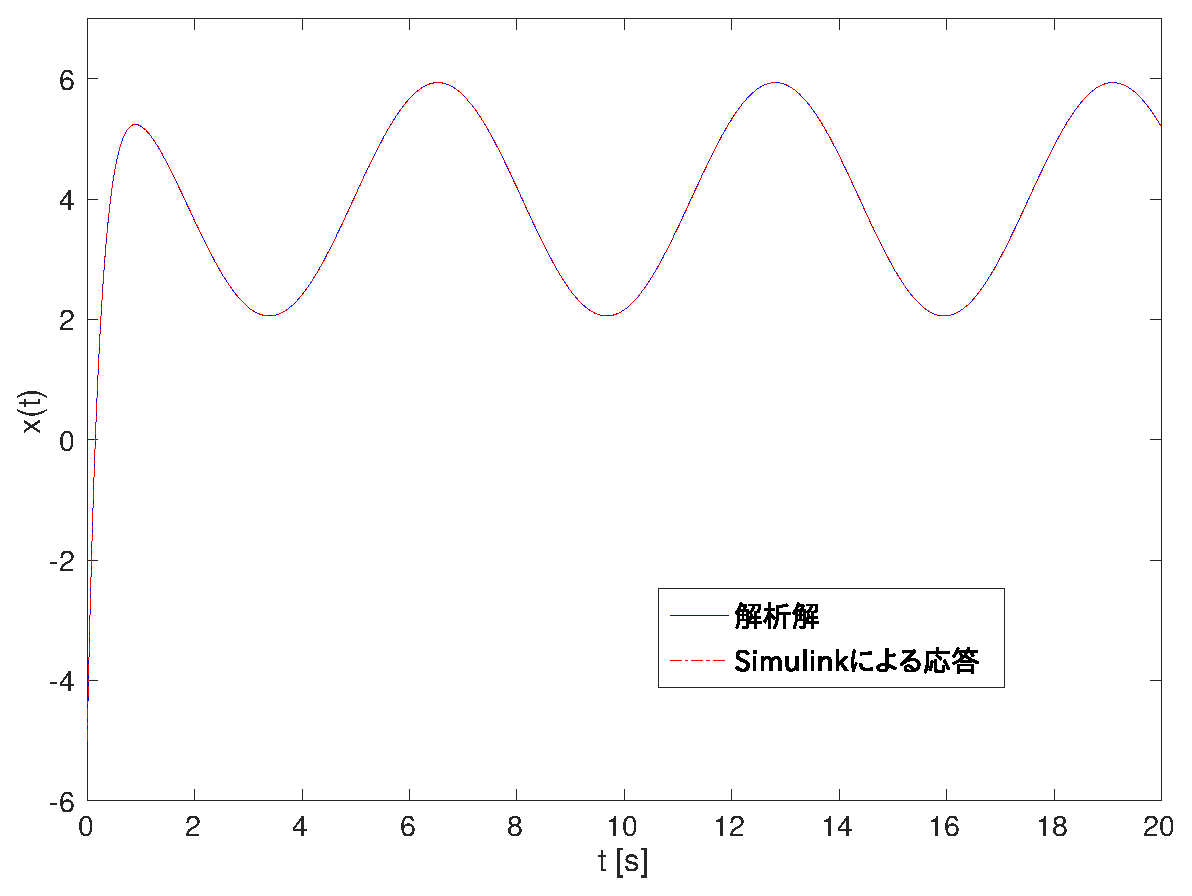
\includegraphics[scale=0.5]{../figure/eps/output2.eps}}
 \caption{Simulinkを用いたシミュレーションの結果}
 \label{Mat_sim}
\end{figure}
%---------------------------------------------
%---------------------------------------------
\newpage
\section{考察・まとめ}
%---------------------------------------------
{\bf Fig.}{\ref{Mat_sim}}より,解析解のグラフとシミュレーションの結果は一致し,定常応答時は$ x(t)= 4 $を中心に振動していることが分かる.
% しかしこれらのグラフには僅かな誤差が見受けられる.
% これは,解析解では厳密な数値解を得ることができるが,シミュレーションでは積分要素の部分を近似的に求めていることが原因ではないかと考えられる.
また,サンプリング周期を小さくすることでシミュレーションの結果を解析解のグラフに近づけられることを確認した.このような変化が生じるのはシミュレーションにおける数値解の算出時に線形近似を用いているためと考えられる.

本課題を通して,シミュレーションにおいてMATLAB/Simulink は高い精度での検証が可能であることが分かった.


% 解析解では厳格な数値解を得ることができるが,シミュレーションではこうした厳密な解が得られないことが原因であるのではないかと考えられる.
% 定常応答時は$ x(t)= 4 $を中心に振動している.
% 本課題では簡単なシステムであった
% 外乱を考慮した際のシミュレーションにも対応
% 解析解の計算をさせることも可能
% ある条件下におけるシミュレーションにおいて高い精度での検証が可能である.ことがわかった.

% 解析解とシミュレーション結果に僅かな差が見られる.これは点のプロットの間隔が0.4周期であるためであると考えられる.
% 解析解では厳密な数値解を得ることができるが,シミュレーションでは積分要素の部分を近似的に求めているため,誤差が蓄積されていくのではないかと考えられる.

% % 図の挿入

% \begin{figure}[b]
%  \begin{center}
%   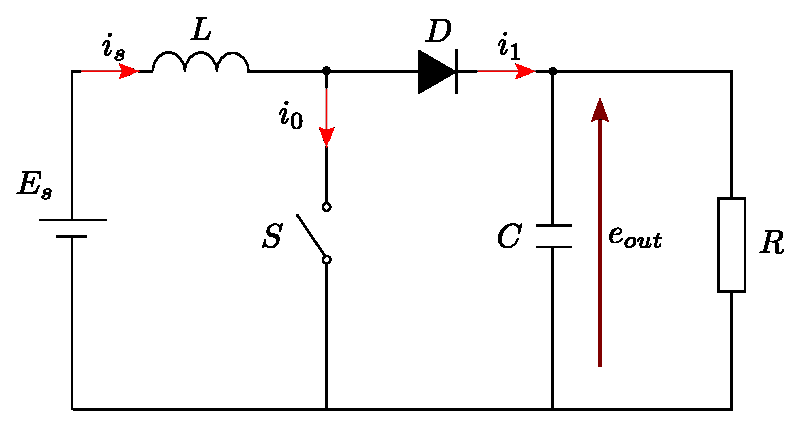
\includegraphics[scale=0.9]{../figure/circuit.eps}
%   \caption{Uncontrolled converter}
%   \label{circuit}
%  \end{center}
% \end{figure}


% % 表の挿入

% \begin{table}[htb]
%   \begin{center}
%     \caption{各素子のパラメータ}
%     \begin{tabular}{c|c|c} \hline
%       定数名[単位] & 記号 & 値 \\ \hline \hline
%       周波数[Hz] & $f_U,f_V,f_W$ & 120 \\ \hline
%                      & $\phi_U$ & $\frac{2\pi}{3}$ \\
%       初期位相角[rad] & $\phi_V$ & $\frac{4\pi}{3}$ \\
%                      & $\phi_W$ & $2\pi$ \\ \hline
%       抵抗[$\Omega$] & $R$ & 10 \\ \hline
%     \end{tabular}
%     \label{param}
%   \end{center}
% \end{table}


% % 図の挿入

% \begin{figure}[tb]
%  \centering
%  \vspace{0.5cm}
%  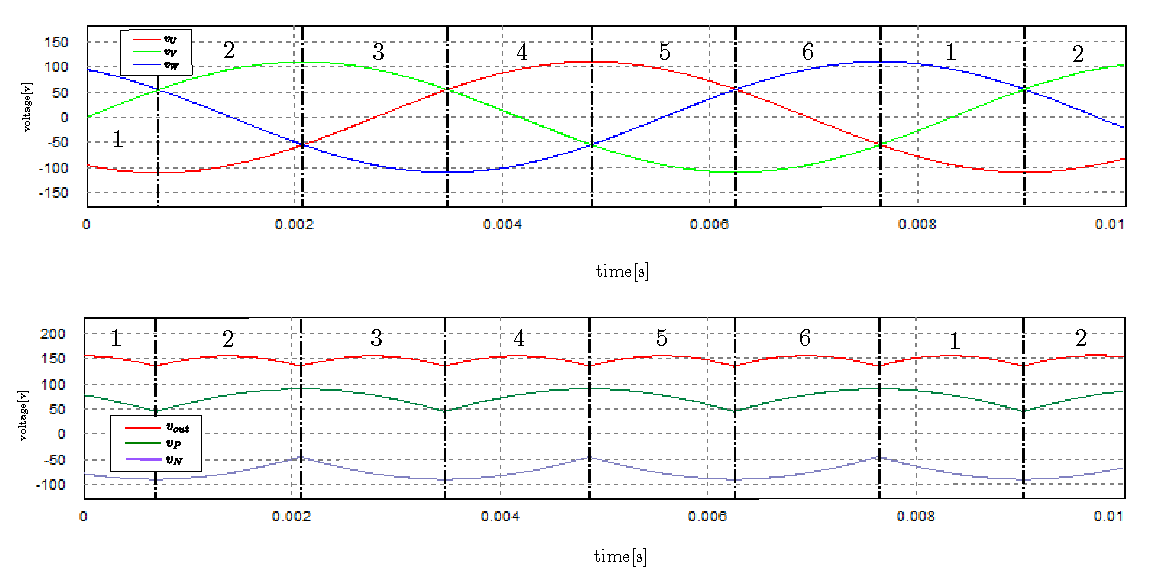
\includegraphics[scale=0.85]{../figure/waves.eps}\\
%  \hspace{0.0cm}
%  % 入力と出力\\
%  % \\
%  % \vspace{1.2cm}
%  % 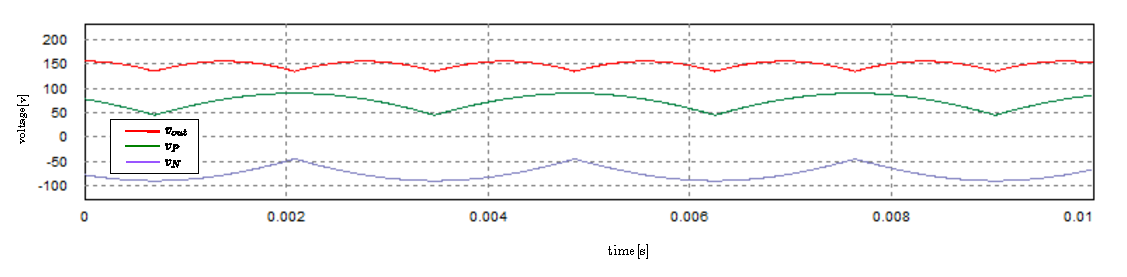
\includegraphics[scale=0.825]{../figure/output.eps}\\
%  % (b) 出力の電位\\
%  % \\
%  \caption{シミュレーションにより得られた各電源電圧(上)と出力電位(下)の波形}
%  \label{wave}
% \end{figure}

% \newpage

% % 図を並べて挿入

% \begin{figure}[tb]
%  \centering
%  \subfloat[区間1における回路動作]{\includegraphics[scale=0.5]{../figure/kukan_1.eps}}
%  \hspace{1.5cm}
%  \subfloat[区間2における回路動作]{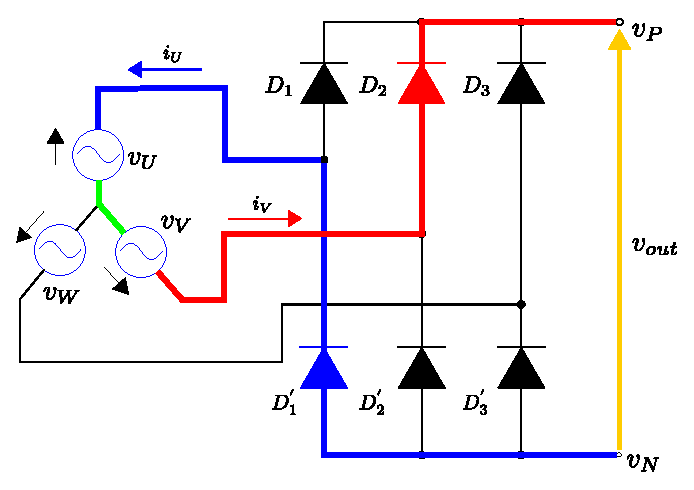
\includegraphics[scale=0.5]{../figure/kukan_2.eps}}
% \\
%  \vspace{0.5cm}
%  \subfloat[区間3における回路動作]{\includegraphics[scale=0.5]{../figure/kukan_3.eps}}
%  \hspace{1.5cm}
%  \subfloat[区間4における回路動作]{\includegraphics[scale=0.5]{../figure/kukan_4.eps}}
% \\
%  \vspace{0.5cm}
%  \subfloat[区間5における回路動作]{\includegraphics[scale=0.5]{../figure/kukan_5.eps}}
%  \hspace{1.5cm}
%  \subfloat[区間6における回路動作]{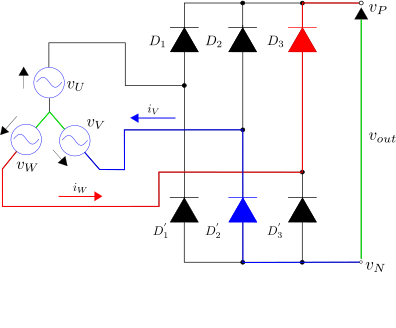
\includegraphics[scale=0.5]{../figure/kukan_6.eps}}
% \\
%  \caption{各区間での回路動作の様子}
%  \label{circuit_kaku}
% \end{figure}

% % 文中へのラベリング
% {\bf Fig. }\ref{circuit_kaku}に示す〜

%---------------------------------------------
% 参考文献
%---------------------------------------------
\begin{thebibliography}{99}
\addcontentsline{toc}{section}{参考文献}
\bibitem{1} 大屋 勝敬,”車両制御特論 MATLAB+Simulink の利用法”,九州工業大学 機械知能工学研究系,2013.
% \bibitem{2} 坪島 茂彦,”誘導電動機 -基礎から制御まで-”,東京電機大学出版局,pp.13-17,2006.
\end{thebibliography}

\end{document}
